
\documentclass[11pt]{beamer}
\usepackage{helvet} %font
\beamertemplatenavigationsymbolsempty
\usetheme{JuanLesPins}
\usefonttheme{structurebold}

\usepackage[french]{babel}
\usepackage[utf8]{inputenc}
\usepackage[T1]{fontenc}
\usepackage{amssymb,amsmath}
\usepackage{tikz}
\usepackage{geometry}
\usepackage{xcolor,colortbl}
\usetikzlibrary{arrows,positioning}
\usepackage{listings}

\AtBeginSubsection[]
{
   \begin{frame}
	\small \tableofcontents[currentsection]
   \end{frame}
}

\newenvironment{slide}[1]{%
\begin{frame}[environment=slide]
\frametitle{#1}
}{%
\end{frame}
}
\setbeamercolor{structure}{fg=red}
\setbeamercolor{frametitle}{bg=black,fg=white}
\definecolor{gris}{gray}{0.6}
\definecolor{grisclair}{gray}{0.9}

\newtheorem{exercice}{Exercice}

\title{Machine Learning I \\ }
\author{Nicolas Bourgeois}
\date{}

\newcommand{\Python}[1]{
	{\small	\lstinputlisting[language=Python]{./#1.py}}
}
\newenvironment{pyenvsmall}
	{ \ttfamily \tiny }
	{\par  }

\newcommand{\Pythonsmall}[1]{
	{\scriptsize \lstinputlisting[language=Python]{./#1.py}}
}
\newcommand{\elimine}[1]{{\textcolor{lightgray}{#1}}}


\begin{document}

\begin{frame}
\maketitle
\end{frame}

\begin{frame}
\small
\tableofcontents
\end{frame}



\section{Atelier python}

\begin{slide}{Nearest Neighbor}

\Python{sklearn1-nn}

\end{slide}

\begin{slide}{Malédiction de la dimension}

Pour que l'estimateur soit efficace, il faut que la distance entre les points soit raisonnablement petite.\\

\vspace{0.3cm}
\pause

Donc le nombre de boules nécessaires pour couvrir croît exponentiellement avec la dimension (le nombre de variables).

\begin{center}

\begin{tikzpicture}
\draw[color=gray](0,0) grid[step=2] (2,2);
\draw(4.5,0) -- (2.5,0);
\draw[color=red] (0.1,0.35) circle (0.2);
\draw[color=red] (0.2,1.15) circle (0.2);
\draw[color=red] (0.1,1.45) circle (0.2);
\draw[color=red] (0.7,0.75) circle (0.2);
\draw[color=red] (0.8,1.85) circle (0.2);
\draw[color=red] (0.9,1.25) circle (0.2);
\draw[color=red] (0.9,0.85) circle (0.2);
\draw[color=red] (1.1,0.4) circle (0.2);
\draw[color=red] (1.15,0.1) circle (0.2);
\draw[color=red] (1.3,1.3) circle (0.2);
\draw[color=red] (1.4,1.15) circle (0.2);
\draw[color=red] (1.7,1.8) circle (0.2);
\draw[color=red] (0.3,0.4) circle (0.2);
\draw[color=red] (0.35,1.15) circle (0.2);
\draw[color=red] (0.55,2) circle (0.2);
\draw[color=red] (0.7,0.35) circle (0.2);
\draw[color=red] (0.73,0.56) circle (0.2);
\draw[color=red] (1.6,0.1) circle (0.2);
\draw[color=red] (1.78,0.9) circle (0.2);
\draw[color=red] (1.33,1.15) circle (0.2);
\draw[color=red] (1.89,1.65) circle (0.2);
\draw[color=red] (0.89,1.45) circle (0.2);
\draw[color=red] (0.26,1.2) circle (0.2);
\draw[color=red] (0.7,0.7) circle (0.2);

\draw[color=red] (2.7,0) circle (0.2);
\draw[color=red] (3,0) circle (0.2);
\draw[color=red] (4.11,0) circle (0.2);
\draw[color=red] (3.2,0) circle (0.2);
\draw[color=red] (3.65,0) circle (0.2);
\end{tikzpicture}

\end{center}

\end{slide}

\begin{slide}{Régression linéaire}

\Python{sklearn2-reglin}

\end{slide}

\begin{slide}{Régression linéaire}

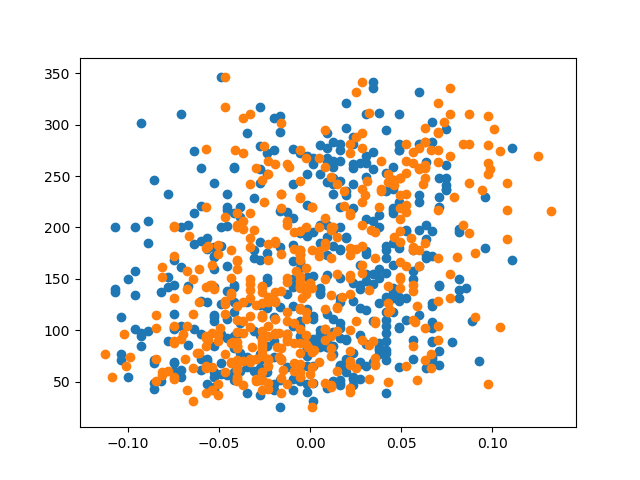
\includegraphics[scale=0.5]{diabete}

\end{slide}

\begin{slide}{Régression logistique}

\Python{sklearn3-reglog}

\end{slide}

\begin{slide}{Régression logistique}

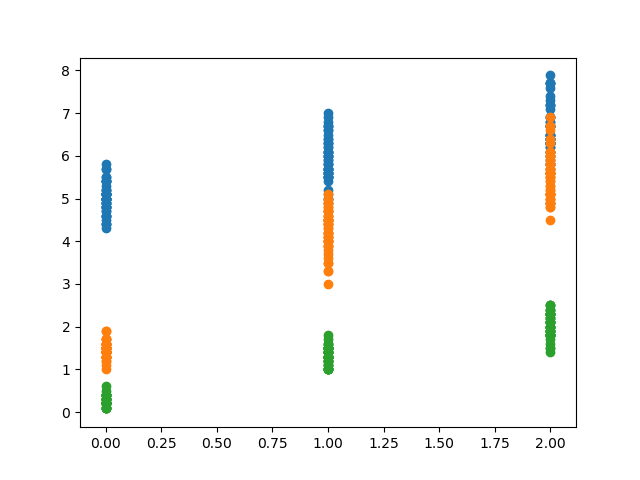
\includegraphics[scale=0.5]{logiris}

\end{slide}

\begin{slide}{SVM}

\Python{sklearn4-svm}

\end{slide}

\begin{slide}{SVM}

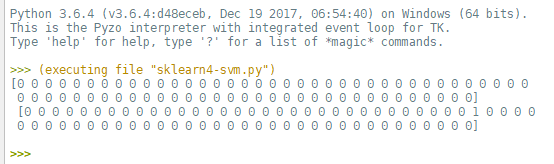
\includegraphics[scale=0.5]{sksvm}

\end{slide}

\end{document}
